\documentclass[11pt,a4paper]{article}
\usepackage[left=2cm,right=2cm,top=2cm,bottom=3cm]{geometry}
\usepackage{fontspec,polyglossia}
\setdefaultlanguage{russian}
\setotherlanguage{english}
\defaultfontfeatures{Ligatures=TeX}
\setmainfont{cmunrm.otf}[Path=fonts/,BoldFont=cmunbx.otf,ItalicFont=cmunti.otf,BoldItalicFont=cmunbi.otf]
\setmonofont{cmuntt.otf}[Path=fonts/,BoldFont=cmuntb.otf,ItalicFont=cmunit.otf,BoldItalicFont=cmuntx.otf]
\newfontfamily\cyrillicfonttt{cmuntt.otf}[Path=fonts/,BoldFont=cmuntb.otf,ItalicFont=cmunit.otf,BoldItalicFont=cmuntx.otf]
\usepackage{graphicx,float,booktabs,tabularx,array,enumitem,setspace,longtable}
\usepackage[unicode,hidelinks]{hyperref}
\setlength{\parindent}{0pt}
\setlength{\parskip}{0.2\baselineskip}
\setlength{\emergencystretch}{2em}
\setlength{\LTpre}{5pt}
\setlength{\LTpost}{5pt}
\setlist{nosep,topsep=3pt}
\setcounter{tocdepth}{2}
\newcolumntype{L}[1]{>{\raggedright\arraybackslash}p{#1}}
\newcolumntype{Y}{>{\raggedright\arraybackslash}X}
\newcommand{\code}[1]{\texttt{\detokenize{#1}}}
\begin{document}
\hypersetup{pageanchor=false}
\begin{titlepage}
    \centering
    Федеральное государственное автономное\\
    образовательное учреждение высшего образования\\
    \textbf{«Национальный исследовательский университет ИТМО»}\\

    \vfill

    \textbf{Практическая работа}\\
    \vspace{0.5\baselineskip}
    Пользовательские сценарии\\
    \vspace{0.5\baselineskip}
    AI Knowledge Agent\\
    \vspace{0.5\baselineskip}
    Из диалога с ИИ в личную базу знаний

    \vfill

    \begin{flushright}
    Выполнили:\\
    Чэнь Хаолинь P3316 407960\\
    Су Лянхуа P3308 407956\\
    Чжун Цзяцзюнь P3310 407959
    \end{flushright}

    \vspace{4\baselineskip}
    \centering
    г. Санкт-Петербург, 2026
\end{titlepage}

\hypersetup{pageanchor=true}
\setstretch{0.95}
\tableofcontents
\newpage
\setstretch{1}



\section{Введение}

Цель работы состоит в том, чтобы описать, как пользователь превращает диалог с ИИ в заметки для личной базы знаний. Для этого нужно выделить группы пользователей, составить не менее двух историй для каждой группы, выбрать истории для MVP и описать обмен информацией между пользователем и системой. Сценарии должны передавать содержание сообщений и решений без названий элементов интерфейса и способов управления ими.


\section{Продукт и целевая аудитория}

AI Knowledge Agent превращает диалоги с ИИ в структурированные заметки в Obsidian. В них сохраняются темы, связанные понятия, вопросы и объяснения, которые нужны для повторения и дальнейшей работы. Перед сохранением система сообщает план, после выполнения сообщает результат.


\subsection{Группа A. Студенты и самостоятельные учащиеся}

\textbf{Контекст.} Изучают программирование, ИИ и другие предметы с помощью длинных диалогов. Используют или готовы использовать Obsidian для личных заметок.


\textbf{Проблема.} Нужные объяснения остаются в истории переписки. Перечитывать весь разговор долго; при ручном конспектировании теряются вопросы и исправленные заблуждения.


\textbf{Цель.} Получить краткий учебный материал с понятной структурой. Сохранить, что именно было непонятно и как это объяснялось в диалоге.


\subsection{Группа B. Разработчики и технические специалисты}

\textbf{Контекст.} Обсуждают с ИИ технологии, алгоритмы и способы решения рабочих задач. Накапливают личную техническую базу знаний.


\textbf{Проблема.} Полезные сведения распределены по разным разговорам. Ручное перенесение занимает время, а механическое сохранение каждого термина создает множество разрозненных заметок. При пополнении базы возникают повторы и противоречия.


\textbf{Цель.} Получить технические заметки с понятной структурой и связями, использовать их в работе и контролировать изменения в своей базе.


\subsection{Основание сегментации}

Группы выделены по основной цели: понять и запомнить материал либо применять технические знания в работе. Один человек может относиться к обеим группам. Описание аудитории основано на гипотезах, а не на результатах интервью. Для проверки гипотез нужно обсудить с представителями каждой группы реальные примеры сохранения диалогов.


Общая ценность продукта для обеих групп - сократить ручную обработку диалогов и получить контролируемый результат в личной базе знаний.



\clearpage
\section{User Story и выбор MVP}

Для каждой группы составлены три истории. Здесь используется отдельная нумерация от US-01 до US-06.


\subsection{Группа A. Учебные цели}

\textbf{US-01 | MVP | Сценарий S1}

\nopagebreak[4]

Я как студент хочу получить структурированную заметку из учебного диалога с ИИ, чтобы повторять материал без перечитывания всей переписки.


\textbf{US-02 | MVP, упрощенный вариант | Сценарий S1}

\nopagebreak[4]

Я как самостоятельный учащийся хочу сохранить свое исходное заблуждение вместе с объяснением из диалога, чтобы при повторении понимать, в чем состояла моя ошибка.


\textbf{US-03 | После MVP, Phase 3}

\nopagebreak[4]

Я как учащийся с накопленной базой заметок хочу связывать новые знания с уже изученными понятиями, чтобы видеть их место в общей системе знаний.


\subsection{Группа B. Рабочие и технические цели}

\textbf{US-04 | MVP | Сценарий S2}

\nopagebreak[4]

Я как разработчик хочу организовать связанные понятия из технического диалога в заметки и разделы с понятными связями, чтобы повторно использовать материал без множества разрозненных записей.


\textbf{US-05 | После MVP, Phase 3}

\nopagebreak[4]

Я как технический специалист хочу дополнять существующую заметку новыми сведениями из диалога, чтобы развивать накопленные знания и избегать повторного описания одного понятия.


\textbf{US-06 | MVP | Сценарии S1 и S2}

\nopagebreak[4]

Я как разработчик, ведущий личную базу знаний, хочу узнать предполагаемые изменения и разрешить их до сохранения, чтобы контролировать содержание своей базы. Эта потребность также относится к группе A.


\subsection{Почему выбраны эти истории}

US-01, US-02, US-04 и US-06 охватывают весь путь: передать диалог, получить организованные знания, понять план, разрешить сохранение и узнать результат. US-02 в MVP охватывает только явно выраженные вопросы, заблуждения и объяснения при надежно определенных участниках диалога.


\textbf{Граница MVP.} Выбран объем второго этапа проекта: создание новых заметок в \code{inbox/}, базовая проверка повторов, связи между новыми заметками, обнаружение конфликтов и обязательное разрешение пользователя на сохранение. Обновление старых заметок, связи между старыми и новыми знаниями, восстановление версий и автономное перепланирование относятся к последующим этапам. Текущая версия проекта шире выбранного учебного MVP.



\clearpage
\section{Сценарий S1. Учебный диалог становится заметкой}

\textbf{Истории:} US-01, US-02, US-06. \textbf{Пользователь:} учащийся из группы A.


\textbf{Ситуация.} После обсуждения RAG с ИИ пользователь хочет сохранить объяснение и свое исправленное заблуждение. В исходном разговоре он предполагал, что в запрос модели передается вся база данных, и получил объяснение этого заблуждения.


\textbf{Предусловия.} Личная база знаний и модель настроены; сохранение в \code{inbox/} разрешено. Участники исходного диалога определены достаточно надежно. Для этого примера подходящей заметки о RAG при базовой проверке не найдено.


Реплики описывают обмен сведениями и решениями. Система может сообщать несколько результатов подряд; отдельный ответ пользователя на каждый из них не требуется.


{\small\setlength{\tabcolsep}{5pt}\renewcommand{\arraystretch}{1.15}
\begin{longtable}{L{9mm}L{26mm}L{\dimexpr\textwidth-6\tabcolsep-35mm\relax}}
\caption{Обмен информацией в сценарии S1}\\
\toprule
\textbf{Шаг} & \textbf{Участник} & \textbf{Передаваемая информация} \\
\midrule\endfirsthead
\toprule
\textbf{Шаг} & \textbf{Участник} & \textbf{Передаваемая информация} \\
\midrule\endhead
\bottomrule\endfoot
1 & Пользователь & «Передаю мой учебный диалог о RAG для сохранения полезных знаний в личной базе». Содержание разговора включает вопрос, исходное предположение пользователя и последующее объяснение ИИ. \\[5pt]
2 & Система & «В диалоге выделена тема RAG. Найдены определение, описание процесса и объяснение исходного заблуждения. Вопрос пользователя и ответ ИИ различимы; эти сведения можно сохранить вместе». \\[5pt]
3 & Система & «Предлагаю создать в inbox/ заметку RAG: определение, основные этапы, исходное заблуждение и объяснение из диалога. Эти части относятся к одной теме, поэтому отдельные заметки для каждого фрагмента не нужны. Сохранение еще не выполнено; требуется ваше разрешение». \\[5pt]
4 & Пользователь & «Разрешаю сохранить заметку по этому плану». \\[5pt]
5 & Система & «Создана заметка inbox/RAG.md. В ней сохранены выделенные сведения и связь с исходным диалогом. Файл повторно прочитан: сохранение и структура проверены. Существующие заметки не изменены». \\[5pt]
\end{longtable}}

\subsection{Результат и критерии успешного завершения}

\begin{itemize}
\item Пользователь получает одну учебную заметку, соответствующую заявленной теме.
\item Исходное заблуждение обозначено как позиция пользователя, а объяснение - как содержание ответа ИИ.
\item Сохранение происходит после разрешения пользователя.
\item Отчет содержит сведения о созданной заметке и результате проверки.

\end{itemize}
\textbf{Возможные отклонения:} повторный диалог, неясные роли, отсутствие пригодных знаний, отказ от плана или ошибка сохранения. Их продолжения описаны в разделе 6.


Сценарий описывает ожидаемый обмен информацией, а не результаты испытаний. Проверка сохранения и структуры не доказывает достоверность исходного объяснения ИИ.



\clearpage
\section{Сценарий S2. Связанные технические знания}

\textbf{Истории:} US-04, US-06. \textbf{Пользователь:} разработчик из группы B.


\textbf{Ситуация.} В одном диалоге обсуждались Transformer, Attention, Self-Attention и Multi-Head Attention. Пользователь хочет получить материал для дальнейшей работы и избежать разрозненных заметок на каждый термин.


\textbf{Предусловия.} База и модель настроены. Диалог содержит достаточно подробное самостоятельное объяснение Attention. В этом примере базовая проверка не выявила препятствий для создания запланированных новых заметок.


{\small\setlength{\tabcolsep}{5pt}\renewcommand{\arraystretch}{1.15}
\begin{longtable}{L{9mm}L{26mm}L{\dimexpr\textwidth-6\tabcolsep-35mm\relax}}
\caption{Обмен информацией в сценарии S2}\\
\toprule
\textbf{Шаг} & \textbf{Участник} & \textbf{Передаваемая информация} \\
\midrule\endfirsthead
\toprule
\textbf{Шаг} & \textbf{Участник} & \textbf{Передаваемая информация} \\
\midrule\endhead
\bottomrule\endfoot
1 & Пользователь & «Передаю технический диалог о Transformer и механизмах внимания для организации знаний в моей базе». \\[5pt]
2 & Система & «Найдена группа связанных понятий: Transformer, Attention, Self-Attention и Multi-Head Attention. Attention подробно объясняется как самостоятельное понятие; два его варианта можно описать внутри этой темы». \\[5pt]
3 & Система & «Предлагаю создать две заметки в inbox/: Transformer и Attention. В Attention войдут разделы Self-Attention и Multi-Head Attention; заметки будут связаны между собой. Причина такого деления: сохранить общее описание архитектуры отдельно от подробного материала о внимании и не дробить варианты механизма на отдельные записи». \\[5pt]
4 & Система & «План предполагает только создание новых заметок. Существующие материалы не изменяются. Сохранение еще не выполнено; требуется ваше разрешение». \\[5pt]
5 & Пользователь & «Разрешаю сохранить эти две заметки с предложенной структурой и связью». \\[5pt]
6 & Система & «Созданы inbox/Transformer.md и inbox/Attention.md. Разделы вариантов внимания включены в Attention. Файлы и ссылки повторно проверены; в отчете указаны созданные заметки и результаты проверки». \\[5pt]
\end{longtable}}

\subsection{Результат и критерии успешного завершения}

\begin{itemize}
\item Получены связанные технические заметки, а не четыре записи по числу терминов.
\item Система объясняет, почему одни понятия стали заметками, а другие - разделами.
\item План охватывает только новые заметки и выполняется после разрешения пользователя.
\item Итоговый отчет позволяет сопоставить запланированный и фактический результат.

\end{itemize}
\textbf{Другой объем материала.} В этом примере содержание разделено на две заметки. Для более короткого диалога может быть достаточно одной заметки с разделами. Число файлов зависит от содержания; система объясняет свое решение.


Если в разговоре есть еще одна несвязанная тема, система сообщает о ней отдельно и не объединяет ее с этим материалом только потому, что сведения находились в одном диалоге.



\clearpage
\section{Альтернативные ветви S1 и S2}

Эти ветви могут возникнуть в обоих сценариях. Система сообщает статус обработки и указывает, нужно ли решение пользователя.


\paragraph{A1. Этот диалог уже передавался}

\textbf{Система:} «Этот диалог уже есть в истории обработки. Можно завершить текущую попытку или повторить анализ; повторный анализ сам по себе не разрешает создание дубликатов».


\textbf{Пользователь:} «Повторный анализ не нужен».


\textbf{Итог:} текущая попытка завершается без новых заметок. Если пользователь все же запрашивает повторный анализ, после него снова требуется план и разрешение на сохранение.


\paragraph{A2. Нет знаний, пригодных для сохранения}

\textbf{Система:} «В разговоре найдены только ситуативные реплики либо сведения, которые нельзя уверенно выделить как самостоятельные знания. Новые заметки не созданы; причина пропуска указана».


\textbf{Пользователь:} «Передам другой диалог, содержащий нужное объяснение».


\textbf{Итог:} текущая обработка завершена без сохранения. Другой диалог обрабатывается как новый материал.


\paragraph{A3. Неясно, кому принадлежит заблуждение}

\textbf{Система:} «Участников диалога не удалось определить достаточно надежно. Личное заблуждение вам не приписано; это ограничение указано в результатах анализа».


\textbf{Пользователь:} «Не разрешаю сохранение этой попытки; подготовлю диалог с обозначенными участниками».


\textbf{Итог:} попытка прекращена. Уточненный материал можно передать для нового анализа.


\paragraph{A4. Найдено противоречие или совпадение с имеющейся записью}

\textbf{Система:} «Найдена существующая запись, которая может повторять или противоречить новому материалу. Сообщаю, какие сведения требуют проверки. Автоматическое объединение и изменение старой заметки не входят в этот MVP; спорное сохранение приостановлено».


\textbf{Пользователь:} «Не разрешаю выполнять этот план; сначала проверю исходные материалы».


\textbf{Итог:} план отклонен, существующая запись не изменена. Базовая проверка MVP не гарантирует обнаружение всех смысловых повторов. Эта ветвь описывает действия после обнаружения проблемы.


\paragraph{A5. Пользователь не согласен с планом}

\textbf{Пользователь:} «Не разрешаю сохранять предложенный результат».


\textbf{Система:} «План отклонен. Запланированные изменения не выполнены».


\textbf{Итог:} завершение без сохранения. Редактирование отдельных действий плана в этот учебный MVP не включено.


\paragraph{A6. Сохранение или проверка результата завершились ошибкой}

\textbf{Система:} «Задача не завершена успешно. Сообщаю, какие действия выполнены, что не удалось сохранить или проверить и какие материалы требуют сверки перед повторной попыткой».


\textbf{Пользователь:} «Проверю указанный результат перед новой попыткой».


\textbf{Итог:} система не сообщает об успешном завершении. Автоматическое восстановление относится к расширенной версии и не требуется для этого сценария MVP.



\clearpage
\section{Блок-схема обмена информацией}

Общий путь для историй US-01, US-02, US-04 и US-06. На схеме показаны передаваемые сведения и решение пользователя. Подробные альтернативные ветви приведены в разделе 6.


\begin{figure}[H]\centering
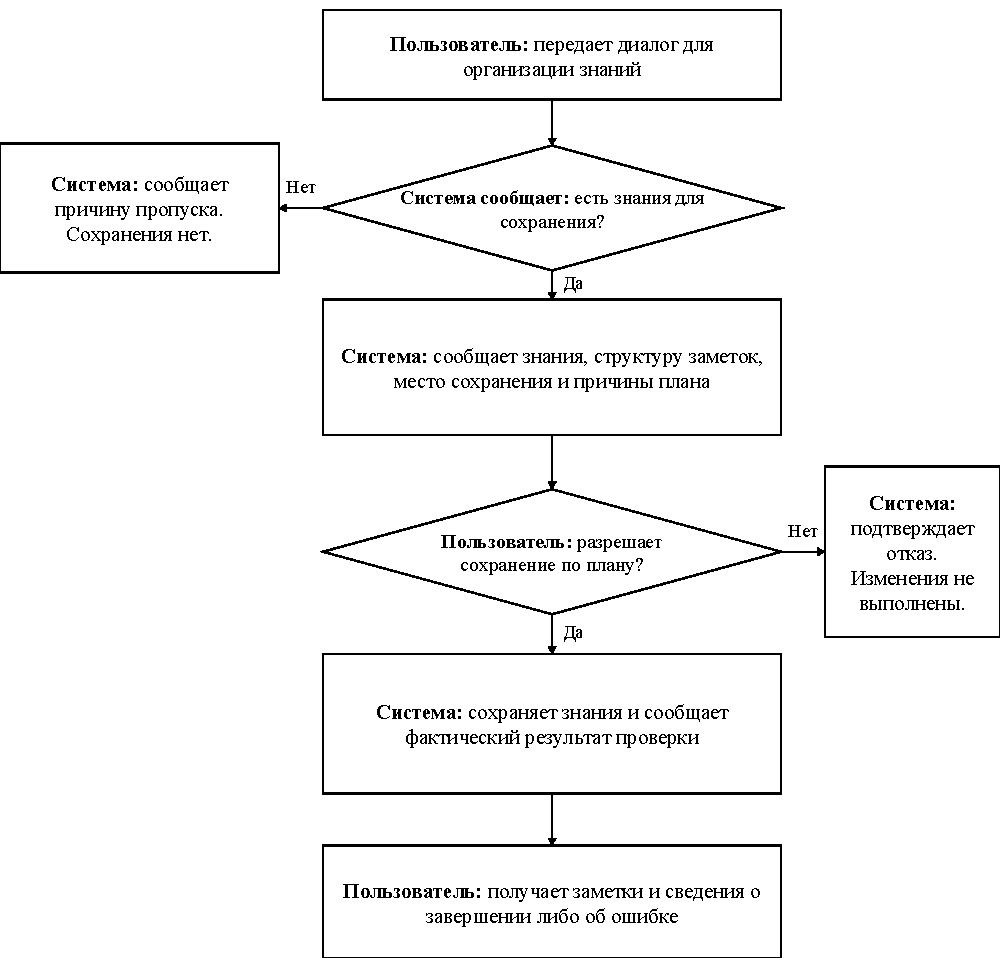
\includegraphics[width=\textwidth]{figures/information-flow.pdf}
\caption{Обмен информацией между пользователем и системой}
\end{figure}

\textbf{Что предоставляет пользователь:} исходный диалог и решение о разрешении сохранения.


\textbf{Что возвращает система:} выделенные знания, обоснованный план, статус выполнения и фактический результат. При проблеме система сообщает ее причину и то, какое решение или уточнение требуется.


\textbf{Граница ответственности:} пользователь решает, подходит ли результат для его базы. Система выполняет разрешенную задачу и проверяет сохраненные файлы.



\clearpage
\section{Агентная система и ее компоненты}

ИИ-агент объединяет языковую модель, инструменты, управление контекстом и процесс выполнения задачи. Он получает цель, предлагает план, выполняет разрешенные действия через инструменты и проверяет результат. В AI Knowledge Agent цель состоит в том, чтобы превратить диалог в заметки для личной базы знаний.


\subsection{Основные компоненты}

\begin{itemize}
\item \textbf{Языковая модель (LLM).} Понимает содержание диалога, выбирает знания для сохранения и предлагает структуру заметок.
\item \textbf{Инструменты.} Читают и ищут заметки, сохраняют новые файлы, проверяют их структуру и ссылки.
\item \textbf{Управление контекстом.} Передает модели нужные части исходного диалога, связанные заметки и состояние задачи. Длинные диалоги обрабатываются по частям.
\item \textbf{Архитектура.} Связывает этапы анализа, планирования, подтверждения, выполнения и проверки. Программа контролирует права записи и обработку ошибок.

\end{itemize}
\subsection{Сравнение с LLM и обычной программой}

\begin{table}[H]\centering\small
\caption{Сравнение способов обработки задачи}
\setlength{\tabcolsep}{4pt}\renewcommand{\arraystretch}{1.1}\setlength{\abovecaptionskip}{5pt}
\begin{tabularx}{\textwidth}{L{0.13\textwidth}YYY}
\toprule
\textbf{Аспект} & \textbf{Чат с LLM без инструментов} & \textbf{Программа на заданных правилах} & \textbf{AI Knowledge Agent} \\
\midrule
Обработка содержания & Формирует ответ по запросу & Применяет заранее заданные правила & Модель понимает диалог, оценивает знания и их связи \\[2pt]
План & Может описать план текстом & Порядок действий определяется правилами & Модель предлагает структуру заметок и план сохранения по содержанию диалога \\[2pt]
Выполнение & В основном возвращает текст & Выполняет предусмотренные операции & Инструменты выполняют разрешенный план \\[2pt]
Результат & Ответ или совет & Результат предусмотренной функции & Заметки в Obsidian и отчет о проверке \\[2pt]
\bottomrule\end{tabularx}\end{table}

Обычная программа тоже может вызывать инструменты и хранить состояние. В нашем проекте модель принимает смысловые решения и предлагает план, а программа управляет его выполнением и проверкой. Чат с инструментами также может обладать агентными функциями.


В проекте используется заданный рабочий процесс с ограниченной самостоятельностью модели. В зависимости от содержания система предлагает одну заметку, несколько связанных заметок или пропуск материала. В MVP каждое сохранение требует разрешения пользователя. Проверка файлов подтверждает результат сохранения, но не истинность всех утверждений в исходном диалоге.


\section{Заключение}

Для двух групп пользователей составлены шесть историй; четыре выбраны для MVP. Два основных сценария и шесть альтернативных ветвей описывают подготовку учебных и технических заметок, решения пользователя и условия завершения задачи. Модель предлагает план, а программа контролирует разрешение на запись, сохранение и проверку файлов.


\end{document}
